\cotefile{16}

\scanpage{17}
\figure{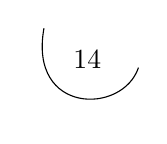
\begin{tikzpicture}[x=1cm,y=1cm]
\node at (0,0) {\mspage{14}};
\draw (-.55,.4) .. controls (-.75,-.7) and (.45,-.7) .. (.65,-.1);
\end{tikzpicture}}
\uline{Cor} Soit $\mathcal E$ un anneau gradué, \inserted{\figure{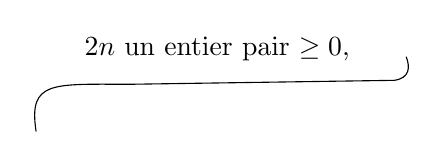
\begin{tikzpicture}[x=1cm,y=1cm]
\node at (0,.35) {$2n$ un entier pair $\geq0$,};
\draw (-2.3,-.7) .. controls (-2.4,-.05) and (-2.1,-.1) .. (-1.1,-.1) --(2.25,-.05) .. controls (2.45,-.02) and (2.45,.12) .. (2.4,.25);
\end{tikzpicture}}} et soit $L\in\mathcal E^{(2)}$.
S'il existe un hom d'anneaux gradués
\[
u:\Phi\longrightarrow\mathcal E
\]
tel que $u(\mathbf L)=L$, et tel que les $u(\boldsymbol\pi_i)=\pi_i$ définissent la graduation de $\mathcal E$ par $(1.3)$, alors un tel $u$ est uniquement déterminé, et les $\pi_i$ sont déterminés de façon unique, en termes de la structure \inserted{\uline{d'anneau}} graduée de $\mathcal E$ par les conditions $(1.1)$ et $(1.3)$.
\inserted{Si on se donne $\pi_i$ satisfaisant les conditions \deleted{\unsure{En l'absence des} $\pi_i$},}
\margin{\figure{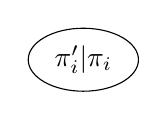
\begin{tikzpicture}\node at (0,0) {$\unsure{\pi'_i|\pi_i}$};\draw (0,0) ellipse (.7cm and .4cm);\end{tikzpicture}}}
l'existence de $u$ équivaut alors : \deleted{l'existence} validité, pour tt $0\leq i\leq n$, de la condition
\[
\text{``}\ \exists w_i\in\mathcal E^{-(2n-2i)}\text{ tel que}\quad(w_iL^{n-i}-1)\pi_{\deleted{i}\inserted{2n-i}}\deleted{=0}\text{''}=0,
\]
et \deleted{alors} le système des $\Lambda=u(\boldsymbol\Lambda)$, \deleted{et} $\pi_{i,\alpha}=u(\boldsymbol\pi_{i,\alpha})$ est alors caractérisé (en termes de $L$ et des $\pi_i$) par les équations $(6.14)$.
\margin{Ou encore : $\exists$ un module fidèle $M^*$ sous $\mathcal E^*$ tel que \unsure{par} \unsure{sa|la} graduation \unsure{coïncide} .... (\unsure{donc ceci pour tt}). \deleted{\unsure{Si on dit}} \unsure{Id du précédent}.}
De la donnée des $\pi_i$, l'existence de $u$ équivaut à l'existence d'un module \uline{gradué} fidèle sous $\mathcal E^*$, \deleted{tel que} $\mathcal E^*$ (\unsure{définie par les} $\pi_i\in\operatorname{End}(M^*)$), et tel que \figure{\begin{tikzpicture}[x=.35cm,y=.35cm,baseline]
\fill (0,0) ellipse (.09 and .045);
\fill (.5,.06) ellipse (.065 and .05);
\fill (.8,.07) ellipse (.07 and .045);
\fill (1.15,.12) ellipse (.09 and .04);
\fill (1.5,.15) ellipse (.055 and .05);
\draw[line width=.8pt] (1.9,.17) .. controls (2.05,.23) and (2.08,.23) .. (2.2,.18);
\draw[line width=.8pt] (2.5,.2)--(2.8,.21);
\fill (4.4,.22) circle (.13);
\end{tikzpicture}}

\uline{Question} Si on ne se donne \uline{pas} la graduation de $\mathcal E$ à priori,
\inserted{\figure{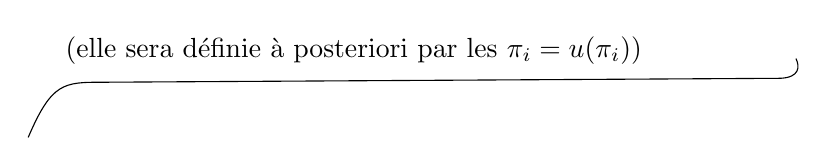
\begin{tikzpicture}[x=1cm,y=1cm]
\node[anchor=west] at (0,.35) {(elle sera définie à posteriori par les $\pi_i=u(\boldsymbol\pi_i)$)};
\draw (-.35,-.75) .. controls (-.05,-.05) and (.1,-.05) .. (.6,-.05) --(9.2,.0) .. controls (9.45,.01) and (9.45,.15) .. (9.4,.25);
\end{tikzpicture}}}
serait-il vrai qu'il y a au plus un hom $\Phi\longrightarrow\mathcal E$ tel que $u(\mathbf L)=L$ !

\figure{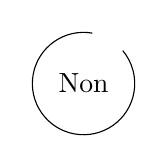
\begin{tikzpicture}\node at (0,0) {Non};\draw (80:.65cm) arc[start angle=80,end angle=400,radius=.65cm];\end{tikzpicture}}, déjà dans le cas $n=1$, $2n=2$, où il y a une base de $\Phi$ formée de $\pi_0,\pi_1,\pi_2,L,\Lambda$, et où $\mathbb Z[L]$ n'est que $\mathbb Z+\mathbb ZL$ ! Il faut donc se donner en $=$ temps \uline{$L$ et les $\pi_i$}.
\mspage{16}

\scanpage{18}
8) Soit maintenant $\mathcal E^*$ un anneau gradué, \deleted{muni de} tel qu'il existe $L\in\mathcal E^{(2)}$ satisfaisant aux \uline{conditions de Lefschetz} (\deleted{de} les conditions du corollaire du n\textsuperscript{o} précédent). On dit que $\mathcal E^*$ est un ``anneau \deleted{d'opérateurs Lefschetzien,}\inserted{de correspondances Lefschetzien}'' (\unsure{cette|celle-ci} \deleted{\illegible{3}} \deleted{\unsure{avec le système}} \unsure{au n\textsuperscript{o}|de n\textsuperscript{o}} (pair) qu'un système de Lefschetz), et $L$ un de ses ``éléments de Lefschetz''.
\deleted{\unsure{En dehors} $(\unsure{\varphi(\Phi)=\mathcal E^*})$}
L'élt $\Lambda$ associé est \deleted{\unsure{appelé|dit}} ``l'élément \deleted{\unsure{adjoint pour}} \deleted{\unsure{anti}}\inserted{co.}Lefschetzien'' associé à $L$.
(NB. À noter que $L$ se déduit de $\Lambda$ comme $\Lambda$ de $L$, par simple symétrie sur les degrés de $\mathcal E^*$ \deleted{$\unsure{\xi_0}$} $-$, et passage à l'anneau opposé --- \deleted{\unsure{transposé}} isom de transposition ---).
\margin{\figure{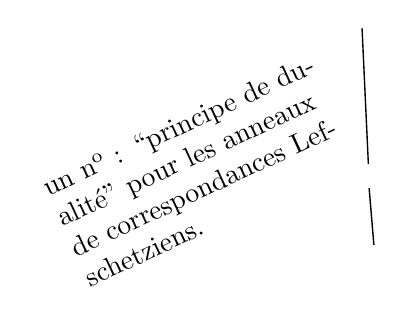
\begin{tikzpicture}
\node[align=left,text width=3.8cm,rotate=25] at (0,0) {un n\textsuperscript{o} : ``principe de dualité'' pour les anneaux de correspondances Lefschetziens.};
\draw[line width=.5pt] (2.05,1.8)--(2.13,.08);
\draw[line width=.5pt] (2.14,-.23)--(2.2,-.95);
\end{tikzpicture}}}

On peut se demander de \uline{caractériser} les \deleted{les} éléments de Lefschetz $L$. Une condition nécessaire, lorsque le nombre $2n$ n'est pas redondant, i.e.
\[
\begin{aligned}
1)\quad&\mathcal E^{(2n)}\neq0\quad\deleted{\unsure{\{}}\quad(\Longrightarrow)\quad1')\ \mathcal E^{(-2n)}\neq0\quad\deleted{\unsure{\}}}\\
&(\Longrightarrow)\quad2)\ \pi_0,\deleted{\unsure{\pi_{2n}}}\neq0\quad\deleted{\unsure{\}}}
\end{aligned}
\]
\margin{\figure{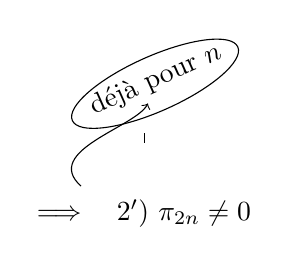
\begin{tikzpicture}
\node[align=left] at (0,0) {$\Longrightarrow\quad2')\ \pi_{2n}\neq0$};
\node[rotate=24] at (.15,1.7) {déjà pour $n$};
\draw[rotate=24] (.8,1.45) ellipse (1.15cm and .35cm);
\draw[->] (-.8,.35) .. controls (-1.3,.8) and (-.1,1.1) .. (.05,1.4);
\draw (.01,1.02)--(.01,.9);
\end{tikzpicture}}}
que
\[
(\Longrightarrow)\quad3)\ L^n\neq0\quad(\Longrightarrow)\quad3')\ \Lambda^{\unsure{n|-}}\neq0\quad\deleted{\Longleftrightarrow}
\]
c'est que l'on ait $L^n\neq0$. On a parfois une réciproque, dans le cas où ($\mathcal E$ étant une \uline{algèbre} sur un anneau commutatif $k$)
\mspage{17}

\scanpage{20}

\deleted{$\unsure{b'}$}
\figure{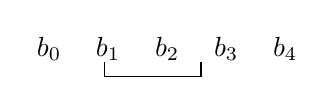
\begin{tikzpicture}
\node at(0,0){$b_0$};\node at(.75,0){$b_1$};\node at(1.5,0){$b_2$};\node at(2.25,0){$b_3$};\node at(3,0){$b_4$};
\draw(.7,-.17)--(.7,-.35)--(1.93,-.35)--(1.93,-.17);
\end{tikzpicture}}
\[
nb_0+(n-1)b_1=\qquad L
\]
\figure{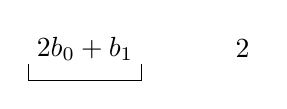
\begin{tikzpicture}
\node at(0,0){$2b_0+b_1$};\node at(2,0){$2$};
\draw(-.72,-.2)--(-.72,-.4)--(.72,-.4)--(.72,-.2);
\end{tikzpicture}}
\[
\lambda^{(n-i)b_i}\qquad\mathcal E^{n-i}\qquad
\mathcal E^{2i}\times\mathcal E^{2n-2i}
\]
\deleted{$\lambda$}
\diagram{\begin{tikzcd}[ampersand replacement=\&]
M^0\arrow[r]\&M^{2n}
\end{tikzcd}}
\deleted{$\Lambda\quad\lambda L\sim$}
\[
L\sim\lambda L\quad\text{alors}\quad\Lambda\sim\frac1\lambda\Lambda
\]
\deleted{$\unsure{\xi|\chi}$}
\[
\Lambda=P(L
\]
\[
\Lambda=\Omega(L)\Delta(L)^{-N}.
\]
\margin{\deleted{$LL'\quad L'^2=LL'$}}
\[
\uline{L'}\quad\uline{LL'}\quad\uline{L^2L'}\quad\deleted{L^4}\quad L^3L'
\]
\[
\left(L^4,\ L'^2-LL',\ L^2L'-L^3,\ L^3L'\right)
\]
\diagram{\begin{tikzcd}[ampersand replacement=\&,column sep=small]
H^0\arrow[rrrr,bend right=20]\&H^1\arrow[rr]\&H^2\&H^3\&H^4
\end{tikzcd}}
\diagram{\begin{array}{c|c|c|c|}
1&L,L'&L^2,LL'&L^3
\end{array}}
\[
L'^3\deleted{\unsure{L}}=L'^2L=L^2L'=L^3
\]
\diagram{\begin{tikzcd}[ampersand replacement=\&,column sep=large]
H^0\arrow[r,dash]\&H^2\arrow[r,dash]\&H^4\arrow[r,dash]\&H^6\\[-1em]
\uuline{\text{rg }1}\&\uuline{\text{rg }2}\&\uuline{\text{rg }2}\&\uuline{\text{rg }1}
\end{tikzcd}}
\[
V\qquad\deleted{\sum V}\qquad\operatorname{Sym}^{\unsure{2}}(V)\mathbin{-}V\mathbin{-}
\]
\[
k
\]
\[
L,L'\qquad L^2=\bar L,\quad L\bar L'=\bar L',\quad \bar L'{}^2=\bar L'
\]
\[
L^{\unsure{4|2}},L',LL'.\qquad L'
\]
\[
\begin{gathered}
L,L'\\
L^2,LL'\qquad L'^2=LL'\\
L^3=L^2L'
\end{gathered}
\qquad
L'^3=LL'^2=L^2L'
\]
\[
\mathbb Z[L]/(L^4)\deleted{\unsure{\mathbb Z}}[L']/L'^2-L^{\prime\prime}
\]

\mspage{19}

\scanpage{22}
$\mathcal E^{2n}$ \deleted{est engendré par} \inserted{admet la \uline{base}} $L_0^n$,
\inserted{(pour un $L_0$ de Lefschetz fixé)}
\deleted{$\mathcal E^{-2n}$ \unsure{engendré} par $\Lambda_0^n$,}
\deleted{pour un choix de $(L,\Lambda)$.}
\deleted{de $\mathcal E^{2n}$, \illegible{2} de $L'$.}
Or.\,--- où, si $L'$ est un autre élément Lefschetzien
\figure{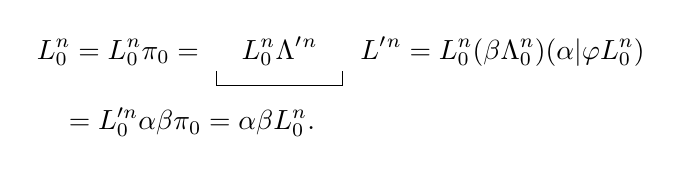
\begin{tikzpicture}
\node[anchor=base east] at(-.9,0){$\displaystyle L_0^n=L_0^n\pi_0=$};
\node[anchor=base] at(0,0){$\displaystyle L_0^n\Lambda'{}^n$};
\node[anchor=base west] at(.9,0){$\displaystyle L'{}^n=L_0^n(\beta\Lambda_0^n)(\unsure{\alpha|\varphi}L_0^n)$};
\draw(-.8,-.15)--(-.8,-.33)--(.8,-.33)--(.8,-.15);
\node[anchor=base west] at(-2.8,-.9){$\displaystyle =L_0^{\prime n}\alpha\beta\pi_0=\alpha\beta L_0^n.$};
\end{tikzpicture}}
ce qui prouve que $\alpha\beta=1$, donc $\alpha$ et $\beta$ inversibles, donc \deleted{\unsure{pour}} $\unsure{L_0^{\prime n}|L_0^n|L'{}^n}$ et $\unsure{\Lambda_0^{\prime n}|\Lambda_0^n|\Lambda'{}^n}$ sont des bases de $\mathcal E^{(2n)}$ et $\mathcal E^{(-2n)}$ respectivement.

D'où
\diagram{\begin{tikzcd}[ampersand replacement=\&,column sep=large]
L^{\unsure{\prime|*}}\ \text{Lefschetzien}\arrow[r,Rightarrow]\&L^n\ \text{\uline{une base de}}\ \mathcal E^{2n}
\end{tikzcd}}
\figure{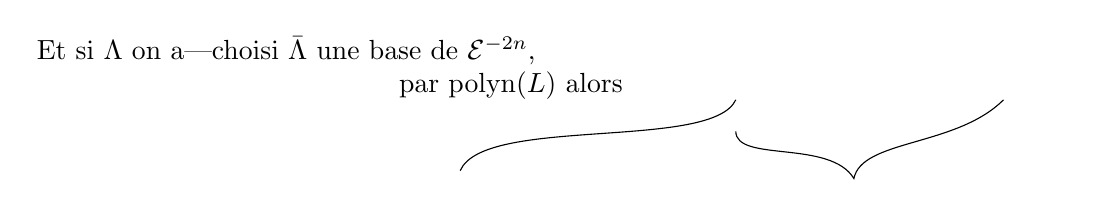
\begin{tikzpicture}[x=1cm,y=1cm]
\node[anchor=west,align=left,text width=13cm] at (0,1.1) {\inserted{Et si $\deleted{\unsure{\Lambda}}$ \unsure{on a|choisi} $\bar\Lambda$ une base de $\mathcal E^{-2n}$,\\\hspace*{4.6cm}par \uline{\unsure{polyn}}$(L)$ alors}};
\draw (5.5,-.2) .. controls (5.8,.5) and (8.7,.05) .. (9,.7);
\draw (9,.3) .. controls (9,-.1) and (10.2,.2) .. (10.5,-.3) .. controls (10.6,.2) and (11.8,.1) .. (12.4,.7);
\end{tikzpicture}}
\margin{?}
On sait prouver une réciproque, dans le cas où \deleted{$\unsure{\mathcal E}$} $\mathcal E$ est projectif de type fini sur $k$. Ça ne marche certainement pas tel quel, p.ex. pour $\mathcal E=\mathcal L(M^*)$, $M^*$ gradué à degrés $0\leq i\leq4$ ---.

Mais ça ne marche pas non plus pour les endom. associés aux élémts de degré $2$ d'une alg. de Lefschetz, pour la dim $6$

$\mathcal E$ engendré par $L,L'$ \inserted{\figure{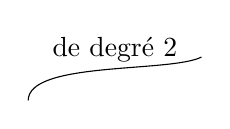
\begin{tikzpicture}
\node at(0,0){de degré $2$};
\draw(-1.1,-.65) .. controls(-1.1,-.15) and(.7,-.3) .. (1.1,-.1);
\end{tikzpicture}}} avec les relations
\[
L^4=0,\quad L'^2-LL'=0,\quad L^2L'-L^3=0,\quad L^3L'=0,\qquad\text{de base}
\]
\diagram{\begin{array}{r c||c||c||c}
&1&L,L'&L^2,LL'&L^3\\\cline{2-5}
\text{deg:}&0&2&4&
\end{array}}
\margin{\figure{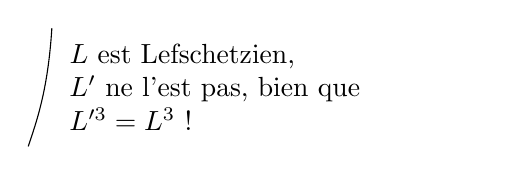
\begin{tikzpicture}
\draw(.3,1.5) .. controls(.25,.7) and(.1,.3) .. (0,0);
\node[anchor=west,align=left,text width=5.1cm] at(.4,.75){$L$ est Lefschetzien,\\$L'$ ne l'est pas, bien que\\$L'^3=L^3$ !};
\end{tikzpicture}}}
\mspage{21}

\scanpage{25}
\begin{flushright}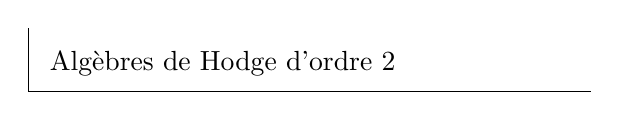
\begin{tikzpicture}
\node[anchor=west] at (0,0) {Algèbres de Hodge d'ordre 2};
\draw (-.15,.45)--(-.15,-.35)--(7,-.35);
\end{tikzpicture}\end{flushright}
\diagram{\begin{array}{ccccc}
H^0&H^1&H^2&H^3&H^4\\
k&V&k\xi+W&\check V&k\xi^2
\end{array}}

$V,W$

\[
\bigwedge^2 V\xrightarrow{\alpha}k\xi+W
\qquad \alpha(x\wedge y)=\varphi(x,y)\xi+\psi(x,y)
\]
\[
\operatorname{Sym}^2(W)\xrightarrow{\beta}k\xi^2
\qquad \beta(xy)=Q(x,y)\xi^2
\]
\margin{$\varphi(x,y)$ forme alternée\par
$\psi(x,y)$ -- appl. bil. alt. dans $W$\par
$Q$ forme bil. sym. sur $W$}

\deleted{\unsure{Point de vue}}
La connaissance de $V,W,\varphi,\psi,\bar Q$ permet de reconstituer $H^*$ :
isom. canonique près.

\[
H^0\times H^i\longrightarrow H^i:\quad\text{clair par}\quad
1.x=x.1=x\qquad\forall x.
\]
\[
H^1\times H^i\longrightarrow H^{i+1}\quad
\left|\begin{array}{ll}
\deleted{\unsure{donc|dont}}\ i=1&xy=\varphi(x,y)\xi+\psi(x,y)\qquad x,y\in V\\
i=2&\begin{array}{l}
x\xi=\xi x=\widetilde\varphi(x):\quad\deleted{\unsure{(*)}}\ y\longmapsto\varphi(y,x)\\
xw=wx=\rho(w,x):\quad y\longmapsto Q(\psi(y,x),w)
\end{array}\quad\left|\begin{array}{l}x\in V\\y\in V\\w\in W\end{array}\right.\\
i=3&xy'=-y'x=\deleted{\unsure{+|-}}\langle x,y'\rangle\xi^2\qquad x\in V,y'\in\check V\\
\deleted{i=4}&\deleted{x\xi^2=0}
\end{array}\right.
\]
\[
H^2\times H^i\longrightarrow H^{j+2}\quad
\left|\quad j=2:\quad\left|\begin{array}{l}
\xi.\xi=\xi^2\\
\xi w=w\xi=0\quad(w\in W)\\
ww'=Q(w,w')\xi^2
\end{array}\right.\right.
\]
\figure{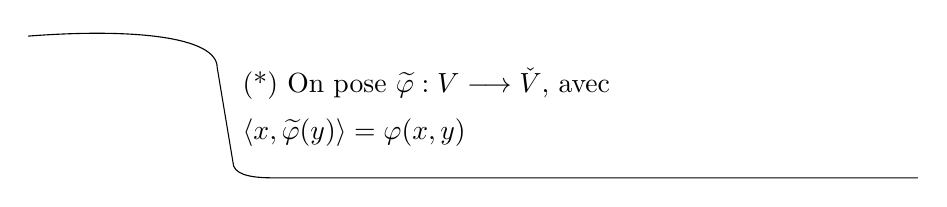
\begin{tikzpicture}[x=1cm,y=1cm]
\node[anchor=west,align=left] at (.2,0) {(*) On pose $\widetilde\varphi:V\longrightarrow\check V$, avec\\[.5em]$\langle x,\widetilde\varphi(y)\rangle=\varphi(x,y)$};
\draw (-2.4,.9) .. controls (-1.1,1) and (0,.9) .. (0,.5) -- (.2,-.7) .. controls (.2,-.85) and (.4,-.9) .. (.7,-.9) -- (8.9,-.9);
\end{tikzpicture}}

Quels que soient les choix de $\varphi,\psi$, on trouve une loi de composition
anticommutative, admettant $1$ comme unité.

\uline{Condition d'associativité} s'écrit $(xy)(tz)=(tx)(yz)$, sous la forme
\figure{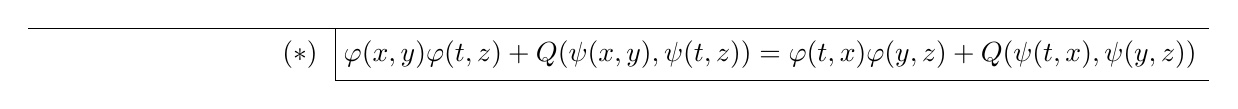
\begin{tikzpicture}
\node[anchor=west,inner sep=0pt] (e) at (0,0) {$\displaystyle\varphi(x,y)\varphi(t,z)+Q(\psi(x,y),\psi(t,z))=\varphi(t,x)\varphi(y,z)+Q(\psi(t,x),\psi(y,z))$};
\node[anchor=east] at (-0.2,0) {$\deleted{\unsure{(*)}}$};
\draw ([xshift=-4cm,yshift=.15cm]e.north west)--([xshift=.15cm,yshift=.15cm]e.north east);
\draw ([xshift=-.1cm,yshift=.15cm]e.north west)--([xshift=-.1cm,yshift=-.15cm]e.south west)--([xshift=.15cm,yshift=-.15cm]e.south east);
\end{tikzpicture}}
\margin{exprime aussi que la forme $(xy)(zt)$ en $xyzt$ est alternée en $y,z$
(donc en \unsure{toutes les var.!|tous les var.!})}

\uline{Condition de Lefschetz}
\[
\xi^2:H^0\simeq H^4\qquad\text{tjrs satisfait}
\]
\[
\xi:H^1\longrightarrow H^3\qquad\text{sss}\quad
\boxed{\varphi\text{ non dégénérée}}
\]

\uline{Condition de Poincaré}
\[
\begin{array}{l}
H^4\simeq k\quad\text{tjrs satisfait}\\
H^0\times H^4\longrightarrow H^4\text{ et }H^1\times H^3\longrightarrow H^4\quad\text{non dég.: }\uline{\text{itou}}\\
H^2\times H^2\longrightarrow H^4\quad\text{non dég sss}\quad\boxed{Q\text{ non dégénérée}}
\end{array}
\]
\mspage{24}

\scanpage{27}
\uline{Cas particulier} Celui où $(xy)(zt)=0$ quels que soient $x,y,z,t$, i.e.
\margin{[i.e. $(H^1)H^3=0$ dans $H^4$ !]}
si l'image de $\alpha:\bigwedge^2V\longrightarrow k\xi+W$ est \deleted{dans} \unsure{un} ss-espace isotrope de $k(\xi)+W$.
\deleted{Par exemple si $W\unsure{\neq0}$, dans le cas alg. clos cela se réalise néc. ainsi : si $W$ est \inserted{de dim} (impaire), alors on peut}

$Q$ non dég. \unsure{étant donné|étant donnée}, et supposons $W\neq0$, il existe (si $k$ \deleted{\unsure{ensuite}} alg. clos disons) une droite isotrope \inserted{$D$} dans $k\xi+W$ qui n'est pas dans $W$, et on prendra pour $\alpha$ \deleted{une forme} définie par une \deleted{forme}\inserted{appl.} bilinéaire \inserted{alt.} non dégénérée \deleted{\unsure{sur}} de $V\times V$ dans $D$: alors $\varphi$ sera aussi non isotrope\ldots

\figure{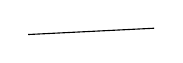
\begin{tikzpicture}\draw (0,0)--(1.6,0.08);\end{tikzpicture}}

Plus généralement, considérons la forme 4-linéaire alternée $\chi$ définie par
\[
xyzt=\chi(x,y,z,t)\xi^2\qquad(x,y,z,t\in V)
\]
Alors la forme \inserted{bilinéaire} induite par la \inserted{forme} $Q\oplus1$ (sur $k\xi+V$) sur $\bigwedge^2 V$ par $\alpha$, qui définit une \deleted{forme} forme linéaire sur
\diagram{\begin{tikzcd}[ampersand replacement=\&,column sep=large]
\operatorname{Sym}^2(\bigwedge^2V)\arrow[rr,bend right=18,"épi."']\&\text{, se factorise en}\&\bigwedge^4V
\end{tikzcd}}
moyennant $\chi$, et donc les données sont les suivantes

a) $V$ vect. (de dim finie) sur $k$

\deleted{b) $\varphi:\bigwedge^2V\longrightarrow k$}

b) $\chi:\bigwedge^4V\longrightarrow k$, définissant une forme bilinéaire symétrique $\chi'$ sur $\bigwedge^2V$

c) un vectoriel $\widetilde W$, avec une forme \deleted{quadratique}\inserted{bil. sym.} $\widetilde Q$, et une application linéaire
\[
\bigwedge^2V\xrightarrow{\alpha}\widetilde W
\]
compatible avec $\chi',Q$ [on dira que $\widetilde W,\widetilde Q$ est une \uline{extension} de la forme $\chi'$]

d) un élément $\xi$ de $\widetilde W$, tel que $Q(\xi,\xi)=1$.

\uline{Conditions de non dégénérescence}
\[
\left|\begin{array}{l}
Q\text{ non dégénérée}\\
\varphi(x,y)=Q(\alpha(x\wedge y),\xi)\text{ non dégénérée}
\end{array}\right.
\]
\mspage{26}

\scanpage{28}
[14] \rule{2cm}{0.4pt}, \uline{Sur quelques points d'algèbre homologique}, Tohoku Math. J., 9 (1957), 119-221.

[15] Hochschild, G., \uline{Local class field theory}, Ann. of Math., 51 (1950), 331-347.

[16] Hochschild, G. and Nakayama, T., \uline{Cohomology in class field theory}, Ann. of Math., 55 (1952), 348-366.

[17] Hochschild, G. and Serre, J.-P., \uline{Cohomology of group extensions}, T.A.M.S., 74 (1953), 110-134.

[18] Lang, S., Abelian Varieties, Interscience Tracts No. 7, 1959, New York.

[19] Nakayama, T., \uline{Cohomology of class field theory and tensor product modules}: I, Ann. of Math., 65 (1957), 255-267.

[20] Ogg, A. P., \uline{Cohomology of abelian varieties over function fields}, Ann. of Math., 76 (1962), 185-212.

[21] Rosenberg, A. and Zelinsky, D., \uline{Amitsur's complex for inseparable fields}, Osaka Math. J., 14 (1962), 219-240.

[22] Serre, J.-P., Corps Locaux, Actualités scientifiques et industrielles No. 1296, 1962, Paris.

[23] \rule{2cm}{0.4pt}, ``Dimension cohomologique'', Notes.at Collège de France, 1962.

[24] \rule{2cm}{0.4pt}, Groupes Algébriques et Corps de Classes, Actualités scientifiques et industrielles No. 1264, 1959, Paris.

[25] \rule{2cm}{0.4pt}, Sur la topologie des variétés algébriques en caractéristique p, Symposium Int. de Top. Alg., 1958, Mexico City.

[26] Shatz, S., \uline{Cohomology of artinian group schemes over local fields}, Ann. of Math., to appear.

[27] Tate, J., \uline{Cohomology of abelian varieties over p-adic fields}, (Cf. Notes by S. Lang, Princeton University, May, 1959.)

\begin{center}45\end{center}
\mspage{27}

\scanpage{29}
\figure{\begin{tikzpicture}[x=1cm,y=1cm]
\node[anchor=west] (a) at (0,3.8) {\deleted{\uline{Exemple} Prenons $\varphi$ non dég.}};
\node[anchor=west,align=left] at (.3,2) {$\begin{array}{l}
\varphi:\bigwedge^2V\longrightarrow k\qquad\text{non dégénérée}\\
\text{i.e. }\varphi\in\bigwedge^2\check V\\
\deleted{\unsure{\text{d'où }\check\varphi\in\bigwedge^2V}}\\
\chi=\varphi^2\in\bigwedge^4\check V\qquad\chi:\bigwedge^4V\longrightarrow k
\end{array}$};
\draw (0,3.4)--(0,.7);
\node[anchor=west] (b) at (0,0) {\deleted{Alors $\chi$ comme forme sur $\bigwedge^2V$ est non}};
\draw (a.east) .. controls +(0.4,0) and +(0,1) .. (8,1.2) .. controls (8,.8) and (10,.9) .. (10,.5)--(10.2,.15);
\end{tikzpicture}}

\uline{Ex} Prenons $\chi'$ non dégénérée, \deleted{\unsure{comme isom.}} $\alpha=\mathrm{id}$ i.e. $\widetilde W=\bigwedge^2V$.

Alors un choix convenable de $\xi\in\widetilde W=\bigwedge^2V$ donne n'importe quelle $\varphi$ voulue, au facteur scalaire, donc n'importe quelle $\check\varphi$ \inserted{$\in\bigwedge^2V$} non dégénérée, au facteur scalaire. Considérons alors $\check\varphi^2$ comme élément de \deleted{$\bigwedge^2V\unsure{\otimes}$} l'algèbre $\bigwedge^*V\otimes\bigwedge^*V$ [en écrivant $\bigwedge^2V\subset V\otimes V$] et $\check\varphi^2$ comme élément de $\bigwedge^2V\otimes\bigwedge^2V\subset\bigwedge^*V\otimes\bigwedge^*V$; le carré de $\check\varphi$ dans $\bigwedge^*V$ \inserted{(quand $\in\bigwedge^2V$)} est l'image de $\check\varphi^{(2)}$ précédent par $\bigwedge^2V\otimes\bigwedge^2V\longrightarrow\bigwedge^4V$. Utilisant la forme $Q:Q_{\chi'}$ définie par $\chi'$, on voit que $\check\varphi^{(2)}$ définit un endom de $\bigwedge^2V$, \uline{soit $u$}. Je dis que l'orbite sous $u$ des éléments $\xi$ et $\check\varphi$ de $\bigwedge^2V$ pourront être infinis, si $\dim V\geq4$ (ou $6$?) ($W$ étant de dim paire) et \deleted{\unsure{de}} \inserted{\unsure{linéairement engendrées et pleines}} de dim non bornée (quand $\dim V$ croissant\ldots).
\deleted{$\unsure{\xi}$}
\mspage{28}

\scanpage{33}
\uline{Formulaire de} $L,\Lambda$.

$X$ variété projective lisse connexe polarisée par $\xi_X\in H^2(X)$, $L_X$ opération de cup-produit associée, $\Lambda_X$ opération de degré $-2$ correspondante, $p_i^X$ les projections de $H^*(X)$ sur les morceaux primitifs $P^i(X)$ pour $0\leq i\leq2n$, $Y$ une section hyperplane lisse de $X$, $\xi_Y\in H^2(Y)$ la self-intersection (induite par $\xi_X$), d'où $L_Y$, $\Lambda_Y$, $p_Y^i$; $\phi:Y\to X$ l'immersion, d'où $\phi^*$ et $\phi_*$.

A) On a
\[
\begin{aligned}
1)\quad&\operatorname{Im}L_X=\bigcap_{0\leq i\leq n}\operatorname{Ker}p_i^X,\qquad
\operatorname{Ker}L_X=\sum_{n\leq i\leq2n}\operatorname{Im}p_i^X,\\
2)\quad&\operatorname{Im}\Lambda_X=\bigcap_{n\leq i\leq2n}\operatorname{Ker}p_i^X\qquad
\operatorname{Ker}\Lambda_X=\sum_{0\leq i\leq n}\operatorname{Im}p_i^X,
\end{aligned}
\]
d'où en particulier les formules
\[
\begin{aligned}
1')\quad&p_i^XL_X=0\text{ si }0\leq i\leq n,\qquad L_Xp_i^X=0\text{ si }n\leq i\leq2n,\\
2')\quad&p_i^X\Lambda_X=0\text{ si }n\leq i\leq2n,\qquad\Lambda_Xp_i^X=0\text{ si }0\leq i\leq n,
\end{aligned}
\]
et en particulier
\[
3)\quad p_n^XL_X=L_Xp_n^X=p_n^X\Lambda_X=\Lambda_Xp_n^X=0.
\]
B) On a
\[
4)\quad\Lambda_XL_X=\mathrm{id}_X-\sum_{\deleted{\unsure{0\leq i\leq n}}\inserted{n\leq i\leq2n}}p_i^X,
\qquad L_X\Lambda_X=\mathrm{id}_X-\sum_{\deleted{\unsure{n\leq i\leq2n}}\inserted{0\leq i\leq n}}p_i^X,
\]
\deleted{d'où compte tenu de 1') et 2') les formules
\[
\begin{aligned}
4')\quad&\Lambda_XL_X^2=\deleted{\unsure{L_X}}\inserted{\left(\mathrm{id}_X-\sum_{0\leq i\leq2n}p_i^X\right)L_X},
\quad L_X^2\Lambda_X=\deleted{\unsure{L_X}}\inserted{L_X\left(\mathrm{id}_X-\sum_{0\leq i\leq2n}p_i^X\right)},\\
4'')\quad&L_X\Lambda_XL_X=\unsure{L_X\left(\mathrm{id}_X-\sum_{0\leq i\leq n}p_i^X\right)
=\left(\mathrm{id}_X-\sum_{n\leq i\leq2n}p_i^X\right)L_X}
\end{aligned}
\]
\inserted{et formules ``transposées''.}}

C) On a
\[
5)\quad\phi_*\Lambda_Y\phi^*=\mathrm{id}_X-\sum_{0\leq i\leq2n}p_i^X
\inserted{\underset{\text{(par 4)}}{=}(\Lambda_XL_X+L_X\Lambda_X)-\mathrm{id}_X+p_n^X}
\]
d'où\inserted{,} \deleted{compte tenu de 4''), 1') et 2')
\[
5')\quad\frac12\Lambda_X L_X^2=\unsure{L_X\phi_*\Lambda_Y\phi^*}
\inserted{\deleted{\phi_*\Lambda_Y\phi^*L_X}}
\qquad L_X^2\Lambda_X=L_X\phi_*\Lambda_Y\phi^*,
\]}
\inserted{posant
\[
(6)\quad T_X=\mathrm{id}_X+\phi_*\Lambda_Y\phi^*,
\]
(donc $\Lambda_XL_X+L_X\Lambda_X=T_X-p_n^X$),}
d'où compte tenu de \deleted{\unsure{4''}}\inserted{3*}) la formule
\[
\deleted{\unsure{6}}\inserted{7})\quad L_X^2\Lambda_X+2L_X\Lambda_XL_X+\Lambda_XL_X^2
=\deleted{\unsure{4L_X(\mathrm{id}_X-\phi_*\Lambda_Y\phi^*)+2(\mathrm{id}_X-\phi_*\Lambda_Y\phi^*)L_X|L_X(\mathrm{id}_X+\phi_*\Lambda_Y\phi^*)+(\mathrm{id}_X+\phi_*\Lambda_Y\phi^*)L_X}}
\inserted{\deleted{\unsure{2L_X+L_X|2L_X+\mathrm{id}L_X}}L_XT_X+T_XL_X},
\]
\inserted{avec $T_X$ \deleted{$\unsure{T_X=\mathrm{id}_X+\phi_*\Lambda_Y\phi^*}$} donné par (6)}

\uline{Corollaire} $(A(X\mathrm{x}X)$ et $C(Y))$ implique $C(X)$.

\margin{On y peut remplacer $A(X\times X)$ par $A^\circ(X\times X)$\par
(condition ``du \unsure{degré|dim} critique'' $H^{(2n)-2}\longrightarrow H^{(2n)+2}$}
\mspage{32}

\scanpage{34}
\uline{Prop}
\[
\left\{\begin{aligned}
P^i(X)&\xrightarrow{\sim}P^i(Y) &&\text{si }i\leq n-2\\
P^{n-1}(X)&\hookrightarrow P^{n-1}(Y) &&\deleted{\text{si }i}\\
P^i(X)&=\operatorname{Ker}\varphi^i &&\text{si }i\geq n
\end{aligned}\right.
\]
\diagram{\begin{tikzcd}[ampersand replacement=\&,column sep=large,row sep=large]
\deleted{\unsure{P}}H^i(X)\arrow[r,"L_X^{n-i+1}"]\arrow[d,"\varphi^i"',"\wr"] \& H^{2n-i+2}(X)\\
H^i(Y)\arrow[r,"L_Y^{n-i\deleted{\unsure{+1}}}"'] \& H^{2(n-1)\unsure{-|+}i}(Y)\arrow[u,"\varphi_{2(n-1)+i}"',"\wr"]
\end{tikzcd}}
\[\left.\vphantom{\begin{matrix}H^i(X)\\H^i(Y)\end{matrix}}\right]\quad\deleted{\unsure{\forall}}\ i\leq n-2\]
\[i\leq n-2\Rightarrow 2(n-1)-i\geq n.\]
\diagram{\begin{tikzcd}[ampersand replacement=\&,column sep=large,row sep=large]
H^j(X)\arrow[d,"\varphi^*"']\arrow[dr,"L_X"] \& \\
H^j(Y)\arrow[r,"\sim"]\&H^{j+2}(X)
\end{tikzcd}}
\[j\geq n\]

\uline{Cor}\qquad Non $\longrightarrow$
\[
\left\{\begin{aligned}
H^*(X)&=\deleted{\sum_i}\coprod_{\substack{i+j\leq n\\i,j\geq0}}L_X^jP^i(X)
=\coprod_{\substack{i+j\leq n-1\\i,j\geq0}}L_X^jP^i(X)\oplus\coprod_{j\geq n}P^j(X)\\
H^*(Y)&=\coprod_{\substack{i+j\leq n-1\\i,j\geq0}}L_Y^jP^i(Y).
\end{aligned}\right.
\]
\uline{Cor}\qquad $\varphi^*$ induit un mor d'objets bigradués
\[
\deleted{\unsure{=}}\coprod_{\substack{i+j\leq n-1\\i,j\geq0}}L_X^jP^i(X)
\longrightarrow H^*(Y)=\coprod_{\substack{i+j\leq n-1\\i,j\geq0}}L_Y^jP^i(Y);\]
\deleted{\unsure{qui est un}}\inserted{c'est} induit un isom sur les morceaux bihomogènes, sauf
\[
L_X^0P^{n-1}(X)=P^{n-1}(X)\longrightarrow\deleted{\unsure{P^{n-1}}}\unsure{\varphi^*}L_Y^0P^{n-1}(Y)=P^{n-1}(Y).
\]
\uline{Cor}\qquad Le noyau de $\varphi^*$ est \inserted{cf. 2 : celui de $L_X$, i.e.}
\[\deleted{\unsure{\sum}}\coprod_{j\geq n}P^i(X)\]
\deleted{(qui est \unsure{un idéal})}. Le conoyau est
\[
\begin{aligned}
E^{n-1}&=H^{n-1}(Y)/\operatorname{Im}H^{n-1}(X)=P^{n-1}(Y)/\operatorname{Im}P^{n-1}(X)\\
&\simeq\operatorname{Ker}\bigl(\varphi_{n-1}:H^{n-1}(Y)\mathrel{\text{---}}H^{n+1}(X)\bigr)
\end{aligned}
\]
\mspage{33}

\scanpage{36}
On aura donc additivement
\[
(\alpha)\qquad H^*(Y)=\coprod_{\substack{i+j\leq n-1\\i,j\geq0}}L_X^jP^i(X)\oplus E^{n-1}.
\]
L'opération
\[\varphi_*:H^*(Y)\longrightarrow H^*(X)\]
s'identifie donc à $L_X$ sur le morceau
\[\coprod_{\substack{i+j\leq n-1\\i,j\geq0}}L_X^jP^j(X)\]
du premier morceau de $(\alpha)$, (et est \deleted{\unsure{un isom}} donc injectif sur ce morceau) et il est \uline{nul} sur le morceau
\[
\deleted{\coprod_{\unsure{0\leq i\leq n-1}}L_X^{\unsure{n-i}}P^i(X)\oplus}E^{n-1},
\]
\deleted{qui correspond \unsure{par l'isom can.} à $\displaystyle\sum_{n-1\leq i\leq2(n-1)}P^i(Y)$}. Ainsi on trouve le

\uline{Corollaire}
\[
\begin{aligned}
\operatorname{Ker}\varphi_*&=\deleted{\coprod_{\unsure{n-1\leq j\leq2n-1}}P^j(Y)\simeq\operatorname{Ker}}E^{n-1}(Y)\\
\operatorname{Im}\varphi_*&=\operatorname{Im}L_X=\bigcap_{0\leq i\leq n}\operatorname{Ker}p_i^X.
\end{aligned}
\]
(la dernière formule, car $H^*(Y)=\operatorname{Im}\varphi^*+E^{n-1}$ et $\varphi_*$ s'annule sur $E^{n-1}$, donc $\operatorname{Im}\varphi_*=\operatorname{Im}\varphi_*\varphi^*\deleted{=I}$, or $\varphi_*\varphi^*=L_X$).
\[
\left\{\begin{aligned}
p_i^X\varphi_*&=0 &&\text{si }0\leq i\leq n\\
p_{j}^X\varphi_*&=\varphi_*p_{j-2}^Y &&\text{si }n+1\leq i\leq2n.
\end{aligned}\right.
\]
On a
\[
\left\{\begin{aligned}
\varphi^*L_X&=L_Y\varphi^*\\
L_X\varphi_*&=\varphi_*L_Y
\end{aligned}\right.
\qquad
\varphi_*\varphi^*=L_X,\quad\varphi^*\varphi_*=L_Y
\]
formule de projection

\margin{\figure{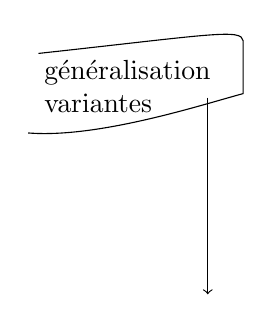
\begin{tikzpicture}[x=1cm,y=1cm]
\node[align=left,anchor=north west] (a) at (0,0) {\deleted{\unsure{généralisation}}\\variantes};
\draw (-.08,-1.05)..controls(.8,-1.12)and(2.1,-.7)..(2.65,-.55)--(2.65,.12)..controls(2.63,.28)and(2.25,.2)..(.05,-.04);
\draw[->] (2.2,-.6)--(2.2,-3.1);
\end{tikzpicture}}}
\deleted{Pour la dernière formule, on note que les deux mbs sont nuls sur $E^{n-1}$, donc il suffit de vérifier
\[
(L_X\varphi_*)\varphi^*=(\varphi_*L_Y)\varphi^*\quad\text{i.e.}\quad
L_X(\varphi_*\varphi^*)=\varphi_*(L_Y\varphi^*)=\inserted{\varphi_*\varphi^*L_X}
\]
car les deux mbs sont $L_X^2$.}
\mspage{35}

\scanpage{38}
A Moyennant l'isom $(\alpha)$, l'opération $L_Y$ s'identifie à $L_X$ sur le morceau
\[
\coprod_{\substack{i+j\leq n-2\\i,j\geq0}}L_X^jP^j(X),
\]
et son noyau est le morceau
\[
\coprod_{\substack{\deleted{i+j}\\i+j=n-1\\i,j\geq0}}\uline{L_X^jP^j(X)}\oplus E^{(n-1)}
=\coprod_{i\geq n+1}P^j(X)\oplus E^{(n-1)}
\]
(qui n'est d'ailleurs autre que $\displaystyle\coprod_{\substack{\deleted{\unsure{i\geq}}\\n\leq i\leq2(n-1)}}P^i(Y)$, comme il se doit). L'opération $\Lambda_Y$ est nulle sur $E^{n-1}$, et coïncide sur le morceau
\[\coprod_{\substack{i+j=n-1\\i,j\geq0}}L_X^jP^i(X)\]
avec $\Lambda_X$. On retrouve \deleted{l'injectivité}\inserted{que le noyau} de $\Lambda_Y$ \deleted{sur} est
\[
\coprod_{0\leq i\leq n-1}P^i(X)+E^{n-1}\simeq\coprod_{0\leq i\leq n+1}P^i(Y),
\]
\deleted{\unsure{donc}} et que $\Lambda_Y$ est injectif sur le reste
\[
=\coprod_{\substack{i+j\leq n-2\\\deleted{i\geq0,j>0}\\i,j\geq0}}L_X^{1+j}P^i(X).
\]
On en déduit
\figure{\begin{tikzpicture}[x=1cm,y=1cm]
\node[anchor=north west,inner sep=0pt,text width=14cm] at (0,0) {\begin{minipage}{14cm}
\deleted{
\[
\left\{\begin{aligned}
\deleted{\unsure{\Lambda_Y\varphi^*=\Lambda_X}}\varphi^*\Lambda_X&=\Lambda_Y\varphi^*+\\
\varphi_*\Lambda_Y&=\Lambda_X\varphi_*
\end{aligned}\right.
\]
Pour la \deleted{dernière}\inserted{prem.} relation, on la vérifie d'abord sur les $P^j(X)$ \inserted{$=$} pour $j\geq n$, \inserted{i.e. les $L_X^{n-i}P^i(X)$ pour $i\leq n-1$)} \deleted{le premier est} y est nul car $\varphi^*$ l'est, le deuxième
}
\end{minipage}};
\draw (-.1,.08)--(8.2,.35);
\draw (-.1,.08)..controls(.05,-.6)and(.1,-1.3)..(-.7,-1.35)--(-.7,-4.35)--(7.4,-4.1)..controls(8.1,-4.1)and(8.1,-3.95)..(8.1,-3.2)--(13.2,-3.05);
\draw (8.5,.5)..controls(9.1,.7)and(9.1,-.7)..(10,-1)..controls(11.1,-1.3)and(13.2,-.9)..(14,-1.2);
\draw (2.7,-1)--(4.8,-3.9);
\draw (5.2,0)--(7.6,-3.1);
\draw (8.8,-.65)--(10.7,-2.85);
\end{tikzpicture}}

\deleted{$\varphi^*\Lambda_X=$}
\[
\left\{\begin{aligned}
\Lambda_Y\varphi^*&=\varphi^*\Lambda_X\left(\operatorname{id}_X-\sum_{n+1\leq j\leq2n}p_X^j\right)
=\left(\operatorname{id}_Y-\sum_{\substack{\deleted{\unsure{n+1}}\\n-1\leq j\leq2(n-1)}}p_X^j\right)\varphi^*\Lambda_X\\
\varphi^*\Lambda_Xp_X^j&=p_Y^{j-2}\varphi^*\Lambda_X\deleted{=p_Y^{j-2}\Lambda_Y\varphi^*}
\qquad\text{si }j\geq n+1.
\end{aligned}\right.
\]
\margin{\[\Lambda_Y^m\varphi^*=\varphi^*\Lambda_X^m(\operatorname{id}-\bar\Sigma)\quad\Longleftarrow\]
pour tt $m$}
\[
\left\{\begin{aligned}
\varphi_*\Lambda_Y&=\left(\operatorname{id}_X-\sum_{0\leq i\leq n-1}p_X^i\right)\Lambda_X\varphi_*
=\Lambda_X\varphi_*\left(\operatorname{id}_Y-\sum_{0\leq i\leq n-1}p_Y^i\right)\\
p_X^i\Lambda_X\varphi^*&=\Lambda_X\varphi^*p_Y^i=p_X^i\varphi_*\Lambda_Y\qquad\text{si }0\leq i\leq n-1.
\end{aligned}\right.
\]
\mspage{37}

\scanpage{40}
On conclut du premier groupe
\[
\varphi_*\Lambda_Y\varphi^*
=\underbrace{\varphi_*\varphi^*\Lambda_X}_{\substack{L_X\Lambda_X\\\Vert\\\operatorname{id}_X-\sum_{0\leq i\leq2n}p_i^X}}
\left(\operatorname{id}_X-\sum_{n+1\leq j\leq2n}p_X^j\right)
=\underbrace{\operatorname{id}_X-\sum_{0\leq j\leq2n}p_X^j}_{q}.
\]
[Plus gén.
\[
\varphi_*\Lambda_Y^m\varphi^*
=\deleted{\sum}\left(\operatorname{id}-\sum_{0\leq i\leq n}p_X^i\right)\Lambda_X^{m-1}
\left(\operatorname{id}-\sum_{n+1\leq j\leq2n}p_X^i\right)
=q\Lambda_X^{m-1}q
\]
où $q=\operatorname{id}-\displaystyle\sum_{0\leq i\leq2n}p_X^i$.
\figure{\begin{tikzpicture}[x=1cm,y=1cm]\draw (0,.3)..controls(1,.5)and(2,.5)..(2.2,.15)..controls(2.3,-.1)and(2.25,-.3)..(2.6,-.3)--(7,-.4);\end{tikzpicture}}

Aussi :
\[
\varphi^*\Lambda_X\varphi_*=\operatorname{id}_Y-\underbrace{p_E}_{\text{projection sur partie évanescente }E^{n-1}}
\]
d'où, en multipliant par $\Lambda_Y$ à gauche, comme $\Lambda_Yp_E=0$
\[
\Lambda_Y=\underbrace{\Lambda_Y\varphi^*}\Lambda_X\varphi_*
=\underbrace{\varphi^*\Lambda_X(\operatorname{id}_X-\sum_{n+1\leq j\leq2n}\overbrace{p_X^j)\Lambda_X}^{\substack{0\\\Vert}}}\varphi_*
\]
donc
\[\boxed{\Lambda_Y=\varphi^*\Lambda_X^2\varphi_*}\]
Donc $C(X)$ \deleted{\unsure{équivaut}}\inserted{implique} $C(Y)$.

Soit $p_X^{i,j}$ les projections sur $L_X^jP^i(X)$ $(i+j\leq n,\ i,j\geq0)$.

Alors
\[
\varphi_*p_Y^{i,j}\inserted{L}\varphi^*=p_X^{i,j+1}
\qquad\text{pour }i+j\unsure{<|\leq}n-1,\quad i,j\geq0\quad\deleted{\unsure{algébrique|quelconque}}
\]
\margin{$L?$}
donc la condition $D(Y)$ implique que les $p_X^{i,j}$ sont algébriques pour $\unsure{\forall}\ i+j<n$, $i\geq0$ et \uline{$j\geq1$}, i.e. les seuls \unsure{rest. en susp.} sont les \uline{$p_X^i$ pour $0\leq i\leq2n$}. Mais
\mspage{39}

\scanpage{41}
\begin{center}-5-\end{center}

is the identity functor. Again since the question is local on $X$, and $L$ is coherent, we write an exact sequence
\diagram{\begin{tikzcd}[ampersand replacement=\&]
0\arrow[r]\&L'\arrow[r]\&\mathcal O_X^p\arrow[r]\&L\arrow[r]\&0
\end{tikzcd}},
with $L'$ also coherent. This gives an exact sequence
\diagram{\begin{tikzcd}[ampersand replacement=\&,column sep=large]
\uline{\operatorname{Hom}}(\mathcal O_X^p,M)\arrow[r]\&\uline{\operatorname{Hom}}(L',M)\arrow[r]\&\uline{\operatorname{Ext}}^1(L,M)\arrow[r]\&0
\end{tikzcd}},
which shows that $\uline{\operatorname{Ext}}^1(L,M)$ is coherent (resp. quasi-coherent), using the case $i=0$ applied to $L'$. We also get isomorphisms for all $i>1$,
\[
\uline{\operatorname{Ext}}^i(L,M)\cong\uline{\operatorname{Ext}}^{i-1}(L',M),
\]
which, by induction on $i$, shows that $\uline{\operatorname{Ext}}^i(L,M)$ is coherent (resp. quasi-coherent) for all $i$.

\uline{Corollary 2.2}: Let $X$ be a locally noetherian prescheme. Let $L^\bullet\in D(X)$ have coherent cohomology, and let $M^\bullet\in D^+(X)$ have coherent (resp. quasi-coherent) cohomology. Assume either
\margin{\figure{\begin{tikzpicture}[x=.3cm,y=.3cm]
\draw (1.35,.45)--(.2,.12)--(.16,-.3)--(.42,-.36)--(.63,-.16);
\end{tikzpicture}}}

a) $L^\bullet\in D^-(X)$,\qquad or

b) $L^\bullet\in D^+(X)$, and there exists an $n_{\unsure{0|o}}\in\mathbb Z$ such that for all $i>n_{\unsure{0|o}}$, and for all coherent sheaves $F$, $\uline{\operatorname{Ext}}^i(F,M^\bullet)=0$.

Then $\uuline{R}\,\uline{\operatorname{Hom}}^\bullet(L^\bullet,M^\bullet)$ has coherent (resp. quasi-coherent) cohomology.

\uline{Proof}: The proof is a good exercise in the use of way-out functors, and will be left to the reader. Note that in case b) the hypothesis on $M^\bullet$ is needed to ensure that the functor
\mspage{40}

\scanpage{42}
Moyennant $C(Y)$, $C(X)$ équivaut à la condition
\[
\left|\begin{gathered}
\forall i\leq n-1,\quad\text{l'hom }\psi_\xi^i:H^i(Y)\longrightarrow H^i(X),\quad\text{inverse à gauche}\\
\text{naturel de }\varphi^i:H^i(X)\mathbin{-}H^i(Y),\quad\deleted{\text{et}}\quad\text{égal : }\Lambda_X\varphi_{i}\mid H^i(Y),\quad\text{est}\\
\text{induit par une classe algébrique.}
\end{gathered}\right.
\]
ou encore :
\[
\left|\quad\Lambda_X\varphi_*\text{ est algébrique}\right.
\]
\deleted{ou encore}\quad N.B. $\Lambda_X\varphi_*$ correspond à une classe de cohomologie
\inserted{$\text{dans }\sum H^{2(n-1)-i}(Y)\otimes H^i(X)=H^{2(n-2)}(X\times Y)=H^{m-1}(X\times Y),\ m=\dim X\times Y$}
sur $X\times Y$, que nous polarisons par $\xi_X\otimes1+1\otimes\xi_Y$.
Or \deleted{$\unsure{\xi_X\otimes1+}$} $L_{X\times Y}(\Lambda_X\varphi_*)$ correspond à
\[
\begin{aligned}
\underbrace{\Lambda_X\varphi_*L_Y}_{\Lambda_XL_X\varphi_*}
 +\underbrace{L_X\Lambda_X\varphi_*}
 &=\deleted{\left(2\operatorname{id}-\sum_{n\leq i\leq2n}p_i^X\right)\varphi_*}\\
 &\inserted{=(\Lambda_XL_X+L_X\Lambda_X)\varphi_*}\\
 &=(\varphi_*\Lambda_Y\varphi^*+\operatorname{id}_X)\varphi_*.
\end{aligned}
\]
\figure{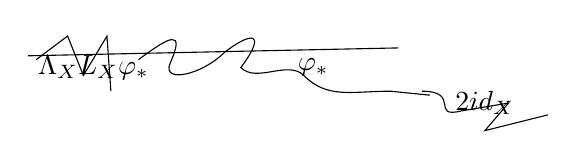
\begin{tikzpicture}[x=1cm,y=1cm]
\node[anchor=west] at (0,0) {$\deleted{\unsure{\Lambda_XL_X\varphi_*}}$};
\node[anchor=west] at (3.3,0) {$\deleted{\varphi_*}$};
\node[anchor=west] at (5.3,-.45) {$\deleted{\unsure{2\operatorname{id}_X}}$};
\draw (0,.15)--(4.7,.25);
\draw (.1,.1)--(.5,.4)--(.7,-.1)--(1,.4)--(1.05,-.3);
\draw (1.4,.1)..controls(1.8,.4)and(2,.5)..(1.8,.05)..controls(1.7,-.2)and(2.2,-.1)..(2.5,.2)..controls(2.9,.5)and(3,.4)..(2.7,.0)..controls(2.9,-.2)and(3.3,.1)..(3.5,-.1)..controls(3.8,-.4)and(4.1,-.3)..(4.6,-.3)--(5.1,-.35);
\draw (5.0,-.3)..controls(5.5,-.3)and(5.1,-.65)..(5.5,-.55)--(6.1,-.45)--(5.8,-.8)--(6.6,-.6);
\end{tikzpicture}}
(car $p_n^X\varphi_*=0$)

Donc est algébrique. Donc on trouve
\[
C(X)\Longleftrightarrow[C(Y)\text{ et }A^0(X\times Y)]
\]
puis de proche en proche
\[
C(X)\Longleftrightarrow\bigl(A^0(X\times Y)\text{ et }A^0(Y\times Z)\text{ et }A^0(Z\times T)\mathbin{-}\mathbin{-}\bigr)
\]
\deleted{$X\times Y,\ Y\times$}\quad
$X\supset Y\supset Z\supset T\mathbin{-}\mathbin{-}$ \unsure{pour une} suite décroissante de sections hyperplanes non singulières.

\figure{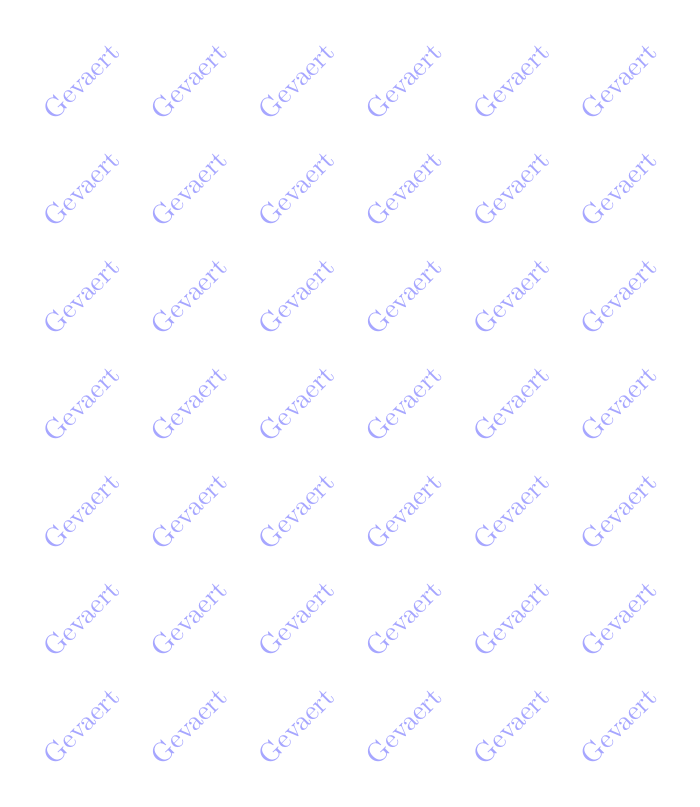
\begin{tikzpicture}[x=.65cm,y=.65cm]
\node[rotate=45,text=blue!35] at (0.0,12.600000000000001){Gevaert};
\node[rotate=45,text=blue!35] at (2.1,12.600000000000001){Gevaert};
\node[rotate=45,text=blue!35] at (4.2,12.600000000000001){Gevaert};
\node[rotate=45,text=blue!35] at (6.300000000000001,12.600000000000001){Gevaert};
\node[rotate=45,text=blue!35] at (8.4,12.600000000000001){Gevaert};
\node[rotate=45,text=blue!35] at (10.5,12.600000000000001){Gevaert};
\node[rotate=45,text=blue!35] at (0.0,10.5){Gevaert};
\node[rotate=45,text=blue!35] at (2.1,10.5){Gevaert};
\node[rotate=45,text=blue!35] at (4.2,10.5){Gevaert};
\node[rotate=45,text=blue!35] at (6.300000000000001,10.5){Gevaert};
\node[rotate=45,text=blue!35] at (8.4,10.5){Gevaert};
\node[rotate=45,text=blue!35] at (10.5,10.5){Gevaert};
\node[rotate=45,text=blue!35] at (0.0,8.4){Gevaert};
\node[rotate=45,text=blue!35] at (2.1,8.4){Gevaert};
\node[rotate=45,text=blue!35] at (4.2,8.4){Gevaert};
\node[rotate=45,text=blue!35] at (6.300000000000001,8.4){Gevaert};
\node[rotate=45,text=blue!35] at (8.4,8.4){Gevaert};
\node[rotate=45,text=blue!35] at (10.5,8.4){Gevaert};
\node[rotate=45,text=blue!35] at (0.0,6.300000000000001){Gevaert};
\node[rotate=45,text=blue!35] at (2.1,6.300000000000001){Gevaert};
\node[rotate=45,text=blue!35] at (4.2,6.300000000000001){Gevaert};
\node[rotate=45,text=blue!35] at (6.300000000000001,6.300000000000001){Gevaert};
\node[rotate=45,text=blue!35] at (8.4,6.300000000000001){Gevaert};
\node[rotate=45,text=blue!35] at (10.5,6.300000000000001){Gevaert};
\node[rotate=45,text=blue!35] at (0.0,4.2){Gevaert};
\node[rotate=45,text=blue!35] at (2.1,4.2){Gevaert};
\node[rotate=45,text=blue!35] at (4.2,4.2){Gevaert};
\node[rotate=45,text=blue!35] at (6.300000000000001,4.2){Gevaert};
\node[rotate=45,text=blue!35] at (8.4,4.2){Gevaert};
\node[rotate=45,text=blue!35] at (10.5,4.2){Gevaert};
\node[rotate=45,text=blue!35] at (0.0,2.1){Gevaert};
\node[rotate=45,text=blue!35] at (2.1,2.1){Gevaert};
\node[rotate=45,text=blue!35] at (4.2,2.1){Gevaert};
\node[rotate=45,text=blue!35] at (6.300000000000001,2.1){Gevaert};
\node[rotate=45,text=blue!35] at (8.4,2.1){Gevaert};
\node[rotate=45,text=blue!35] at (10.5,2.1){Gevaert};
\node[rotate=45,text=blue!35] at (0.0,0.0){Gevaert};
\node[rotate=45,text=blue!35] at (2.1,0.0){Gevaert};
\node[rotate=45,text=blue!35] at (4.2,0.0){Gevaert};
\node[rotate=45,text=blue!35] at (6.300000000000001,0.0){Gevaert};
\node[rotate=45,text=blue!35] at (8.4,0.0){Gevaert};
\node[rotate=45,text=blue!35] at (10.5,0.0){Gevaert};
\end{tikzpicture}}
\mspage{41}

\scanpage{43}
\mspage{- IV - \inserted{977} - \inserted{12} -}
$u:B\longrightarrow A$, où $B=k\inserted{[}[T_1,\ldots,T_r]\inserted{]}$ ($r$ entier quelconque) faisant de $A$ une $B$-algèbre finie, $\uline{m}$ est le seul point de $\operatorname{Spec}(A)$ au-dessus' \unsure{de|du} l'idéal maximal \deleted{\unsure{son}} $\uline{n}$ de $B$ ; \deleted{\unsure{donc}} le morphisme \deleted{$\unsure{{}^a u|\operatorname{Spec}(u)}:\operatorname{Spec}(A)\longrightarrow\operatorname{Spec}(B)$}\inserted{$\operatorname{Spec}(A)\longrightarrow\operatorname{Spec}(B)$} ne peut être non ramifié en $\uline{m}$ que si $A/\uline{n}A$ est un corps, extension séparable de $k$ (17.4.1), ce qui implique que le corps résiduel $K$ de $A$ est une extension séparable de $k$. Si cette condition n'est pas remplie, la conclusion de (18.11.5) ne peut jamais être vérifiée pour $\uline{p}=\uline{m}$, quel que soit l'entier $m$.

(ii) Supposons toujours $\uline{p}\neq\uline{m}$, mais considérons le cas où la condition de (18.11.5) relative à \inserted{l'existence de} l'idéal minimal $\uline{q}$ n'est pas remplie. Soit $\uline{J}$ le noyau de l'homomorphisme canonique $A\longrightarrow A_{\uline{p}}$, autrement dit l'ensemble des annulateurs des éléments de $A-\uline{p}$, et posons $A'=A/\uline{J}$ ; on a nécessairement $\uline{J}\subset\uline{p}$, et si l'on pose $\uline{p}'=\uline{p}/\uline{J}$, l'homomorphisme canonique $A_{\uline{p}}\longrightarrow A'_{\uline{p}'}$ est \uline{bijectif}. En vertu de (18.11.3.3) et de (\uline{0},20.4.12), l'homomorphisme canonique
\deleted{$\unsure{\widehat\Omega^1_{A/k}\otimes_A A'\longrightarrow\widehat\Omega^1_{A'/k}}$}
$\overset{\inserted{\scriptscriptstyle\wedge}}{\Omega}^1_{A/k}\otimes_A A'\longrightarrow\widehat\Omega^1_{A'/k}$ est \uline{surjectif}, donc il en est de même de $(\widehat\Omega^1_{A/k})_{\uline{p}}\longrightarrow(\widehat\Omega^1_{A'/k})_{\uline{p}'}$. D'autre part, l'homomorphisme canonique $A'\longrightarrow A'_{\uline{p}'}$ est par définition \uline{injectif}, et les idéaux \inserted{premiers} minimaux de $A'$ correspondent donc biunivoquement à ceux de $A'_{\uline{p}'}$ ; \deleted{\unsure{donc}}\inserted{par suite} Il y a un idéal minimal $\uline{q}'$ de $A'$ \deleted{\unsure{et|qui}} contenu dans \deleted{\unsure{un}} $\uline{p}'$ et tel que $\dim(A'/\uline{q}')=\dim(A')$. On peut ainsi appliquer (18.11.5) à $A'$ et $\uline{p}'$, et il y a donc un $k$-homomorphisme local $u':B\longrightarrow A'$, avec $B=k\inserted{[}[T_1,\ldots,T_m]\inserted{]}$ tel que le morphisme correspondant \deleted{$\unsure{{}^a u'|\operatorname{Spec}(u')}:$}\inserted{$f':$}$\operatorname{Spec}(A')\longrightarrow\operatorname{Spec}(B)$ soit fini et non ramifié au point $\uline{p}'$. Mais on peut factoriser $u'$ en $B\xrightarrow{u}A\xrightarrow{p}A'$ où \deleted{\unsure{$u$ est injectif et}} $p$ est l'homomorphisme canpnique ; d'autre part, l'injection canonique $\operatorname{Spec}(A')\longrightarrow\operatorname{Spec}(A)$ est un\deleted{e} \deleted{\uline{\unsure{immersion ouverte|immersion fermée}}} \uline{isomorphisme local} au point $\uline{p}'$ en vertu de l'isomorphisme $A_{\uline{p}}\xrightarrow{\sim}A'_{\uline{p}'}$ et de (\uline{I},6.5.4). On voit donc que l'hypothèse a) de (18.11.5) entraîne encore, dans ce cas, l'existence d'un $k$-homomorphisme local $u:B\longrightarrow A$ tel que

\margin{\uline{Vider} (ii) sauf raison sérieuse !}
\mspage{42}

\scanpage{44}
\margin{4.1.67.}
Dear Coates,

I want to add a few more comments to the talk on algebraic cycles and to what I told you on the phone.

I think the best will be to state the index conjecture right after the statement of the main results of Hodge theory, adding that this conjecture will take its whole significance only when coupled with ``conj.A'' in the next paragraph. This will give more freedom in the next paragraph to express some extra relationships between various conjectures, such as $A+\text{index}$ implies $B$.

In c\inserted{h}ar. zero, state some known extra features: index theorem holds, the \deleted{conjectures}\inserted{propositions} $A_{\chi}$ to $D_{\chi}$ are independant of $\chi$ (because of the existence of Betti cohomology, so that these \deleted{conjectures}\inserted{propositions} are equivalent to the corresponding one's for rational cohomology), \deleted{and} $A$ and $C$ are independant of the choosen polarization$_{\mathrm{x}}$ (for $A$ because it is equivalent with $B$, for $C$ because it can be expressed in terms of $A$, $C(X)=(A(X\mathrm{x}X)+A(Y\mathrm{x}Y)+\mathinner{..})$ Thus the \deleted{conjectures}\inserted{conditions} without ambiguity can be called $A(X)$ to $D(X)$, without \deleted{index}\inserted{subscript} $\chi$ and without indication of polarization. Say too that it is known that $C(X)$ is of finite dimension over $\uline{Q}$, \inserted{(}so that $A$ can also be expressed in terms of an equality of dimensions of $C^i$ and $C^{n-1}$\deleted{)}, which again proves it is independant of \hspace{1em}), bu that this is not known in car $p>0$. Contrarily to what I hastily stated in my talk (influenced from my recollections of the car $0$ case) it is not clear to me if in car $p>0$ the \deleted{conjectures}\inserted{conditions} \deleted{$A(X)$} $A_{\chi}(X,\inserted{\xi})$ and $C_{\chi}(X,\inserted{\unsure{\xi}})$ are independant of the polarization $\inserted{\xi}$ ; if you do not find some proof of this independance, then the possible dependance should be pointed out, as well as the fact that \deleted{\unsure{a} priori} we do not have a proof that $A$ to $D$ are independant of $\chi$. Of cour-
\mspage{43}

\scanpage{45}
se, if the index theorem is proved for $X$, then $A_{\chi}(X,\inserted{\unsure{\xi}})=B_{\chi}(X)$ is again independant of the polarization, and analoguous remark for $C_{\chi}(X,\inserted{\unsure{\xi}})$.

When speaking about condition $C_{\chi}(X,\inserted{\unsure{\xi}})$, emphasize at once its stability properties by products (the proof I suggested works indeed) specialization (with possible change of characteristics), hyperplane or more generally linear sections. Give an extra proposition for the relations with the property $A$, via a formal proposition as follows:

\uline{Proposition}\quad Condititions équivalentes sur $X$(varieté \uline{polarisée}):

(i) $C_{\chi}(X)$

(ii) $C_{\chi}(Y)$ et $A_{\chi}(X\mathrm{x}X)^{\deleted{\unsure{0}}}$, \deleted{où l'exposant $^0$}

(ii bis) $C_{\chi}(Y)$ et $A_{\chi}(X\mathrm{x}X)^0$, où l'exposant $^0$ signifie qu'on se borne à exprimer la condition $A$ pour l'homomorphisme en dimension critique
\[
H^{2n-2}\longrightarrow H^{2n+2}.
\]

(iii) $C_{\chi}(Y)$ et $A_{\chi}(X\mathrm{x}Y)$.

(iii bis) $C_{\chi}(Y)$ et $A_{\chi}(X\mathrm{x}Y)^0$, où l'exposant $^0$ signifie qu'on se borne à exprimer la condition $A$ en dimension critique $H^{(2n-1)-1}\longrightarrow H^{(2n-1)+1}$.

(iv) \deleted{Pour tout $\unsure{n|O|0}$} $C_{\chi}(Y)$, et pour tout $i\leq n-1$, l'homomorphisme naturel $H^i(Y)\mathbin{-}H^i(X)$ inverse à gauche de $\varphi^i:H^i(X)\mathbin{-}H^i(Y)$ (induit par $\Lambda_X\varphi_{*}$) est induit par une classe de correspondance algébrique (induisant ce qu'elle veut sur les autres $H^j(Y)$).

(iv bis) $C_{\chi}(Y)$, et pour $j\geq n+1$, l'homomorphisme naturel $H^j(X)\longrightarrow H^{j\inserted{-2}}(Y$ inverse à droite de $\varphi_{j-2}:H^{j-2}(Y)\mathbin{-}H^j(X)$ \deleted{est} (induit par $\varphi^*\Lambda_X$) est induit par une classe de correspondance algébrique (induisant ce qu'elle veut sur les autres $H^i(X)$).

\uline{Corollaire}\quad \unsure{Cés|Ces} conditions équivalent aussi à
\[
\text{(v)}\qquad A_{\chi}(X\mathrm{x}X)^0+A_{\ell}(Y\mathrm{x}Y)^0+A_{\ell}(Z\mathrm{x}Z)^0+\qquad,
\]
où $X\supset Y\supset Z$ est une suite décorissante de sections hyperplanes\inserted{ non sing.}
\mspage{44}

\scanpage{46}

\[
\text{(vi)}\quad A_{\chi}(X\mathrm{x}Y)^0+A_{\chi}(Y\mathrm{x}Z)^0+\mathinner{\ldotp\ldotp\ldotp\ldotp}\ ,\quad\text{avec les mêmes notations .}
\]

Of course, the products and hyperplane sections are endowed with the polarizations stemming from the polarization on $X$. The conditions (v) and (vi) have tthe slight interest that they allow to express the conjecture $A(k)=C(k)$ in terms of $A(T)^0$ for every $T$ of even (resp. odd dimension), where the upper $0$ means that it is sufficient to look at what happens in critical dimensions.

For thenproof of the proposition, I told you already the equivalence of (i) and (ii),(ii bis). The equivalence of (iv) and (iv bis) is trivial by transposition, they \deleted{are of course implied by (i) because of the stabilities because $C_{\chi}(X)$ \unsure{et} $C_{\chi}(Y)$} imply (i) because $H^{2n-i}(X)\to H^i(X)$ is the compositum
\[
H^{2n-i}(X)\mathbin{-}H^{2n-i-2}(Y)\mathbin{-}H^i(Y)\mathbin{-}H^i(X
\]
where the extreme arrows are the ones of (iv bis) and (iv) and the middle one is induced by $\Lambda_Y^{(n-1)-i}$, and they are implied by (iii bis) because of the formula
\[
\deleted{\unsure{\varphi_*\varphi}}\quad(\Lambda_X\varphi_*)L_Y+L_X(\Lambda_X\varphi_*)=(\varphi_*\Lambda_Y\varphi^*+\operatorname{id}_X)\varphi_*\ .
\]
On the other hand $(\mathrm{iii})\Rightarrow(\mathrm{iii\ bis})$ is trivial, and so is $(\mathrm{i})\Longrightarrow(\mathrm{iii})$ because of the stabilities.
\margin{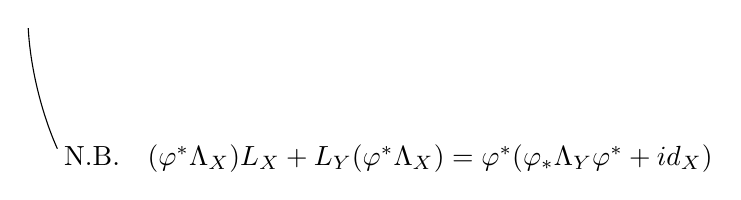
\begin{tikzpicture}[baseline=(nb.base)]\node[anchor=west,inner sep=0pt] (nb) at (0,0) {N.B.\quad $(\varphi^*\Lambda_X)L_X+L_Y(\varphi^*\Lambda_X)=\varphi^*(\varphi_*\Lambda_Y\varphi^*+\operatorname{id}_X)$};\draw (-.45,1.65) .. controls (-.42,1.10) and (-.26,.52) .. (-.08,.12);\end{tikzpicture}}

For the list of the known facts, you can state that :

1) In arbitrary caracteristics, $C(X)$ is known if $\dim X\leq2$, because more generally, it is known that in arbitray dimension $n$, $H^{2n-1}(X)\to H^1(X)$ is induced by an algebraic correspondance class; also, in arbitray dimension, it is known that $\pi_0,\pi_{2n},\pi_1,\pi_{2n-1}$ are algebraic (trivial for the first two, not quite trivial for the two next one's). If $\dim X=3$, it is not known however, even in \unsure{dim|car} $0$, if $C(X)$ or only $D(X)$ hold, nor $A(X)$ and $B(X)$ in car. $p>0$;
\inserted{also if for $1$-cycles, $\tau$-equiv. $=$ num. équivalence $\mathinner{\ldotp\ldotp\ldotp\ldotp}$}

\mspage{45}

\scanpage{47}

By the way, the fact that the $\pi_i$ for a surface are algebraic was pointed out (Tate tells me) by Hodge in Algebraic correspondances between surfaces, Proc. London Math. So\unsure{c|f}. Seeies 2, Vol XLIV, 1938, p.226. It is rather striking that this statement should not have struck the algebraic geometers more, and has fallen into oblivion for \inserted{nearly} thirty years !

2) In car.0, $A(X)$ is known for $\dim X\leq4$. But $A(X)^0$ is not known if $\dim X=5$; the first interesting case would be for a variety $X\mathrm{x}Y$, $X$ of dim 3 and $Y$ a hyperplane section, as this would prove $C(X)$, see above.

Thus the main problems arise already for 1-cycles on threefolds, and partially even in car.0 . Urged by Kleiman\deleted{n}'s question, I wi\deleted{\unsure{h}}\inserted{l}l look again at my old scribbles on that subject (when I pretend to reduce the ``strong'' form of Lefschetz to the ``week'' one). As for the suggestion I made on the phone, to try to get any $X$ as birat\deleted{m}\inserted{i}onally equivalent to a non singular $X'$, which is a spcialisation of a non singular $X''$, itself birationally equivalent to a non singular hypersurface - this cannot work as Serre pointed out, because such an $X$ would have to be simply connected ! Thus if one wants to reduce somehow to the case of hypersurfaces, one will have to work also with singular ones, and see how to reformulate for singular varieties the standard conjectures \ldots

Sincerely your's

\mspage{46}

\scanpage{48}

\margin{6.1.1966}

Dear Coates,

Here a\inserted{\ }few more comments to my talk on the conjectures. The following proposition shows that the conjecture $C_{\chi}(X)$ is independant of the choosen polarization, and has also some extra interest, in showing the part playd by the fact that $H^i(X)$ should be ``motive-theor\deleted{i}etically'' isomorphic to its natural dual $H^{2n-i}(X)$ (as usual, I drop the twist for simplicity).

\uline{Proposition}\quad The condition $C_{1}(X)$ is equivalent also to \inserted{each of} the follwing conditions:

a) $D_{\chi}(X)$ horlds, and for every $i\inserted{{}<n}$, there exists an isomorphism $H^{2n-i}(X)\to H^i(X)$ which is algebraic (i.e. induced by an algebraic correspondance class; we do not make any assertion on what it induces in degrees different from $2n-i$).

b) For every endomorphism $H^i(X)\mathbin{-}H^i(X)$ which is algebraic, the coefficients of the characteristic polynomial are rational, and for every $i\inserted{{}<n}$ there exists an isomorphism $H^{2n-i}(X)\mathbin{-}H^i(X)$ which is algebraic.

Proof. I sketched already how $D_{\chi}(X)$ implies the fact that for an algebraic endomorphism of $H^i(X)$, the coefficients of the characteristic polynomial are rational numbers, Therefore we know that a) implies b), and of course $C_{\chi}(X)$ implies a). It remains to prove that b) implies $C_{\chi}(X)$. Let $u:H^{2n-i}(X)\mathbin{-}H^i(X)$ be the given isomorphism which is algebraic, and $v:H^i(X)\mathbin{-}H^{\unsure{2}n-i}(X)$ \deleted{an}\inserted{the} algebraic isomorphism in the opposite direction, induced by $L_X^{n-i}$. Then $uv=w$ is an automorphism of $H^i(X)$ which is algebraic, and the Hamilton-Cayley formula
\[
u^{b}-\sigma_1(w)u^{b-1}+\ldots+\deleted{\unsure{(-1)|(\pm1)}}(-1)^b\sigma_b(w)=0
\]
(where the $\sigma_i(w)$ are the coefficients of the car. pol. of $w$) whos that $w^{-1}$ is a linear combination of the $w^i$, with coefficients of the type $\pm\sigma_i(w)/\sigma_b(w)$\quad (NB $b=\operatorname{rank}H^i$). The assumption implies

\mspage{47}

\scanpage{49}

that these coefficients are rational, which implies that $w^{-1}$ is algebraic, and so is $w^{-1}u=v^{-1}$, which was to be proved.

NB In char. 0, \deleted{it is} the statement simplifies to: $C(X)$ equivalent to the existence of algebraic isomorphisms $H^{2n-i}(X)\to H^i(X)$,(as the preliminar\deleted{a}y condition in b) is then automatically satisfied). Maybe with some extra care this can be proved too in arbitrary characteristics.

\uline{Corollary}\quad Assume $X$ and $X'$ satisfy condition $C_{\chi}$, and let $u:H^i(X)\mathbin{-}H^{i+2\unsure{\delta|d|j}}(X')$ \inserted{$(\unsure{\delta|d|j}\in\uline{Z})$} be an isomorphism which is algebraic. Then $u^{-1}$ is algebraic.

Indeed, the two spaces can be identified ``algebraically'' (both directions !) to their dual, so taht the transpose of $u$ can be viewed as an isomorphism $u':H^{i+2\unsure{\delta|d|j}}(X')\mathbin{-}H^i(X)$. Thus $u'u$ is an \inserted{algebraic} automorphism \inserted{$w$} of $H^i(X)$, and by the previous argument we see that $w^{-1}$ is algebraic, hence so is $u^{-1}=w^{-1}u'$.

As a consequence, we see that if $x\in H^i(X)$ is such that $u(x)$ is algebraic ($i$ being now assumed to be even), then so is $x$. The same result should hold in fact if $u$ is a monomorphism, the reason being that in this case there should exist a left-inverse which is algebraic; this exists indeed in a case like $H^{n-1}(X)\to H^{n-1}(Y)$ (where we take the left inverse $\Lambda_X\varphi_*$). But to get i\deleted{n}\inserted{t} in general, it seems we need moreover the Hodge index relation. (The complete yoga then being that we have the category of motives which is semi-simple !). Without speeking of motives, and staying down on earth, it would be nice to explain in the notes that $C(X)$ together with the index relation $I(X\mathrm{x}X)$ implies that the ring of correspondance classes for $X$ is semi-simple, and how one deduces from this the existence \deleted{an}\inserted{of} left and right inverses as looked for above.

\mspage{48}

\scanpage{50}

This could be given in an extra paragraph (which I did not really touch upon in the talk), containing also the deduction of the Weil conjectures from the conjectures $C$ and $A$.

A last and rather trivial remark is the following. Let's introduce \deleted{a} variants $A'_{\chi}(X)$ and $A''_{\deleted{\unsure{n}}\inserted{\chi}}(X)$ as follows:

$A'_{\chi}(X):$ if $2i\leq n-1$, any element \inserted{$x$} of $H^i(X)$ whose image in $H^i(Y)$ is algebraic, is algebraic.

$A''_{\chi}(X):$ if $2j\geq n-1$, any \inserted{algebraic} element \deleted{\unsure{of} $H^i(Y)$ whose image in} \inserted{of} $H^{j+2}(X)$ is \deleted{algebraic, is algebraic \unsure{is}} the image of an algebraic element of $H^i(Y)$.

Let us consider also the specifications $A'_{\chi}(X)^0$ and $A''_{\chi}(X)^0$, where we restrict to the \unsure{crittval|critical} dimensions $2i=n-1$ if $n$ odd, $2i=n-2$ if $n$ even. All these conditions are in the nature of ``week'' Lefschets relations, and they are trivially implied by $A_{\chi}(X)$ resp. $C_{\chi}(Y)$ (in the first case, applying $\varphi$ we see that $L_Xx$ is algebraic; in the second, we take $y=\Lambda_Y\varphi^{+}(x)$). The remark then is that these pretend\inserted{ed}ly ``week'' variants in fact imply the full Lefschets relations for al\inserted{ge}braic cycles, namely:

\uline{Proposition}\quad $\unsure{C|A}_{\chi}(X)$ is equivalent to the \unsure{conjunction} $C_{\chi}(Y)+A'_{\chi}(X\mathrm{x} X)^0+A''_{\chi}(X\mathrm{x} X)^0$, hence (by induction) also to the conjunction of the conditions ${A'_{\chi}}^0$ and ${A''_{\chi}}^0$ for all of the varieties $X\mathrm{x} X,Y\mathrm{x} Y,Z\mathrm{x} Z\ \mathinner{\ldotp\ldotp\ldotp\ldotp}\ .$ Analoguous statement with $X\mathrm{x} Y,Y\mathrm{x} Z$ etc instead of $X\mathrm{x} X,Y\mathrm{x} Y$ etc.

This comes from the remark that \deleted{if $X$ is even-dimensional (say a square like $X\mathrm{x} X$) then} $A_{\chi}(X\deleted{\mathrm{x} X})^0$ follows from the conjuction of $A'_{\chi}(X)^0$ and $A''_{\chi}(X)^0$, as one sees by decomposing $L_X^2:H^{2m-2}(X)\to H^{2m+2}(X)$ into
\diagram{\begin{tikzcd}[ampersand replacement=\&,column sep=small]
H^{2m-2}(X)\arrow[r,"\varphi^*"] \& H^{2m-2}(Y)\arrow[r,"\varphi_*"] \& H^{2m}(X)\arrow[r,dash,"L_X"] \& H^{2m+2}\deleted{\unsure{XX|X}}(X)
\end{tikzcd}}
if $\dim X=2m$ is even, and $H^{2m}\deleted{\unsure{(}}{}^{+1-1}(X)\to H^{2m+1+1}(X)$ into
\diagram{\begin{tikzcd}[ampersand replacement=\&,column sep=small]
H^{2m}(X)\arrow[r,dash,"\varphi^*"] \& H^{2m}(Y)\arrow[r,dash,"\varphi_*"] \& H^{2m+2}(X)
\end{tikzcd}}
if $\dim X=2m+1$ is odd.

Sincerely your's

\mspage{49}

\scanpage{51}

\uline{Lemme}\quad Soit $A$ un anneau d'endomorphismes du gpe abélien $H^*(X)$, stable par composantes homogènes (degré \uuline{total}), par transposition. \deleted{et} \inserted{Supposons $\xi\in A$, et} que pour tout $0\leq i<n$, il existe $u_i\in A$, \figure{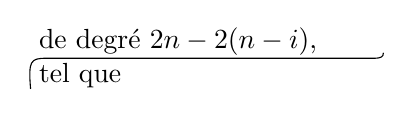
\begin{tikzpicture}[baseline=(t.base)]
\node[anchor=west,inner sep=0pt] (t) at (0,0) {tel que};
\node[anchor=south west,inner sep=0pt] at (0,0.25) {\inserted{de degré $\deleted{2n}-2(n-i)$,}};
\draw (-0.10,-0.17) .. controls (-0.13,0.19) and (-0.10,0.22) .. (0.10,0.22) -- (4.25,0.22) .. controls (4.36,0.22) and (4.38,0.24) .. (4.38,0.29);
\end{tikzpicture}}
\[
u_i\xi^{n-i}:H^i(X)\longrightarrow H^{2n-i}(X)\longrightarrow H^{i}(X)
\]
soit l'identité.
\margin{\figure{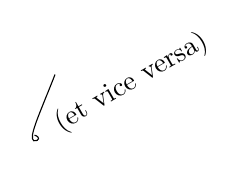
\begin{tikzpicture}[baseline=(v.base)]
\node[anchor=west,inner sep=0pt,rotate=30] (v) at (0,0) {(et vice versa)};
\draw (-0.02,0.65) .. controls (-0.22,0.14) and (-0.36,-0.15) .. (-0.29,-0.19) .. controls (-0.22,-0.20) and (-0.20,-0.14) .. (-0.28,-0.12);
\end{tikzpicture}}}
Alors $A$ contient $L$!, \deleted{les $\pi$} et les projections sur les facteurs élémentaires $\xi^jP^i$ ($i\leq n$, et \deleted{et $i+2j\leq n$ \unsure{ou} $i+2j\leq 2n-i$ \unsure{ou}} $j\leq n-i$)

\uline{Corollaire}\quad Conditions équivalentes :

(i) $L$ Algébrique

(ii) pour tt $1\leq i\unsure{<|\leq}n$, il existe une corr. \uline{alg} induisant $H^{2n-i}(X)\mathbin{-}H^i(X)$ inverse de $J^i$.

\deleted{(iii)} S'il en est ainsi, alors les \deleted{$\unsure{\xi}$} projections sur les facteurs élémentaires de $H^*(X)$, sont algébriques, et les projections $H^*(X)\mathbin{-}H^i(X)$, aussi.

\uline{Dém du lemme.}\quad Comme $A$ stable par transposition, il suffit de regarder les $\xi^jP^i$, pour $i+2j\leq n$. Soit $k=i+2j$. -- procéder par récurrence sur $k$, trivial si $k<0$.

\mspage{50}

\scanpage{52}

Algèbres étales et le différente (4)\hfill Tribu n° 65

§ 2. \uline{Différente.}

\uline{n° 1.}\quad \uline{Idéaux de Filting d'un module} $M$.

Voir thèse de D. Lazard. Lien avec le contenu. Le premier Filting est compris entre $\operatorname{Ann}(M)$ et une de ses puissances.

\uline{n° 2.}\quad \uline{Différente de Kähler.}

On prend pour $B$ une algèbre de \margin{\figure{\begin{tikzpicture}[baseline=(e.base)]
\node[anchor=base,inner sep=0pt] (e) at (0.50,0) {!};
\draw[line width=0.45pt] (0,0.02) -- (0.23,0.02);
\end{tikzpicture}}}p. f. sur $A$ (plus généralement il suffit peut être de supposer que $\Omega_A(B)$ est un $B$-module de p. f.). Par définition la différente de Kähler $\uline{D}_{B/A}$ est le premier idéal de Filting de $\Omega_A(B)$ :

si
\diagram{\begin{tikzcd}[ampersand replacement=\&,column sep=small]
A^p\arrow[r,"u"]\&A^q\arrow[r]\&\Omega_A(B)\arrow[r]\&0
\end{tikzcd}}
, c'est $\operatorname{Im}(\Lambda^q u)$.

La variété des zéros de $\uline{D}_{B/A}$ est l'ensemble des points de ramification. Comportement de $\uline{D}_{B/A}$ par changement d'anneau (c'est trivial).

\uline{n° 3.}\quad \uline{Transitivité.}

Dire ce qu'on sait. Si on a $A\to B\to C$ avec $C$ intersection complète locale sur $B$, la formule de transitivité marche.

\uline{n° 4.}\quad \uline{Lien avec la trace.}

Définir la différente de Dedekind par la trace, et montrer qu'elle coïncide avec celle de Kähler quand $A$ et $B$ sont des anneaux de valuation discrète (il s'agit du gros th. 3 du n° 7, § 2, avec son dévissage, - éventuellement agrémenté des lemmes du n° 6 s'ils n'ont pas été faits dans un chapitre antérieur pour illustrer la notion d'intersection complète. En tous cas on aura dit que si $A$ et $B$ sont réguliers, $A\to B$ est une intersection complète relative. La prop. 11 sera éclairée par le lemme suivant :

``Si $k\to R$ est finie et si $R/\operatorname{rad}(R)$ est étale, alors $R$ monogène ssi les idéaux maximaux de $R$ sont homogènes''.

La prop. 12 est absorbée par le résultat ci-dessus sur les anneaux réguliers.

\uline{n° 5.}\quad \uline{Compléments.}

La ramification modérée du n° 5 (noter que la formule de réduction des traces utilisée en haut de la p. 25 est faite en Alg. VIII, § 11).

Donner la description Kummerienne des extensions totalement et modérément ramifiées (extraire la racine n-ième d'une uniformisante bien choisie ; ceci dans le cas complet); exemple des surfaces de Riemann (ici le groupe de Galois a un générateur canonique $\exp\left(\dfrac{2i\pi}{n}\right)$).

\mspage{51}
